\subsubsection{Schließer}
Damit die Kammer fest verschlossen werden kann, wird die Tür mit sogenannten Kniehebelspanner an den Rahmen gepresst.
Die Kniehebelspanner können nicht direkt am Gestell montiert werden, da ihr Arm zu lang ist und dadurch die Tür nicht mehr geöffnet werden könnte.
\begin{figwindow}[0,r,\includegraphics[scale=1]{image/Schließer1.png},{Schließer}]
Aus diesem Grund wurde aus einem Reststück Aluprofil ein Adapter gebaut und mit einem 3D Drucker ein Winkel gedruckt. In das Loch vom Aluprofil wurde ein Gewinde geschnitten, denn so kann man den Winkel anschrauben.
\end{figwindow}
\vspace{20mm}
\begin{figwindow}[0,l,\includegraphics[scale=1]{image/Schließer2.png},{Winkel}]
Damit der Winkel genau auf das Aluprofil passt, hat dieser eine Grundfläche von 4x4cm. Die Rückseite wird an dem Gestell mit einer M8 Schraube fixiert.
\end{figwindow}
\vspace{40mm}
\begin{figure}[H]
    \centering
    \begin{subfigure}[b]{0.4\textwidth}
        \centering
        \includegraphics[width=\textwidth]{image/geöffnet.png}
        \caption{geöffnet}
        \label{fig:bild1}
    \end{subfigure}
    \hfill
    \begin{subfigure}[b]{0.45\textwidth}
        \centering
        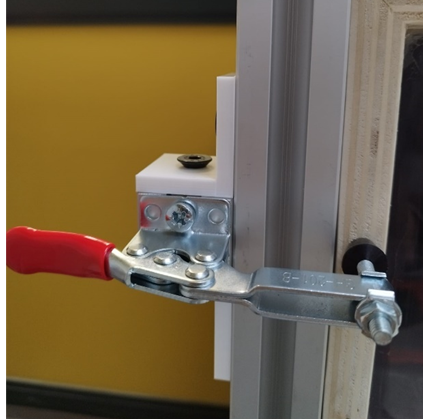
\includegraphics[width=\textwidth]{image/geschlossen.png}
        \caption{geschlossen}
        \label{fig:bild2}
    \end{subfigure}
    \caption{Zustand Schließer}
    \label{fig:zwei_bilder}
\end{figure}